\thispagestyle{empty}
 
Соснин В.В., Балакшин П.В., Шилко Д.С., Пушкарев Д.А., \linebreak Мишенёв А.В., Кустарев П.В., Тропченко А.А. Введение в параллельные вычисления. -- СПб: Университет ИТМО, \the\year. -- \pageref{LastPage}~с. \\

Рецензент: Зилинберг А.Ю., к.т.н., доцент кафедры радиотехнических систем, ФГАОУ ВО <<Санкт-Петербургский государственный университет аэрокосмического приборостроения>>. \\

В пособии излагаются основные понятия и определения теории параллельных вычислений. Рассматриваются основные принципы построения программ на языке <<Си>> для многоядерных и многопроцессорных вычислительных комплексов с общей памятью. Предлагается набор заданий для проведения лабораторных и практических занятий. \\

Учебное пособие предназначено для студентов, обучающихся по магистерским программам направления <<09.04.04 -- Программная инженерия>>, <<09.04.01 -- Информатика и вычислительная техника>>, и может быть использовано выпускниками (бакалаврами и магистрантами) при написании выпускных квалификационных работ, связанных с проектированием и исследованием многоядерных и многопроцессорных вычислительных комплексов.
	%\parРекомендовано к печати Ученым советом факультета компьютерных технологий и управления, 8 декабря 2015 года, протокол №10.\textbf{НЕТ!!!!}

\vspace*{\fill}

\begin{flushright}
    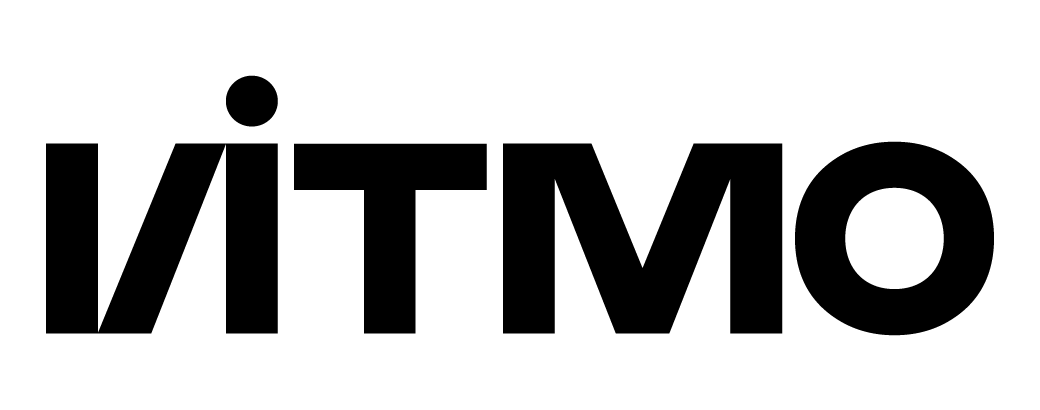
\includegraphics[scale=0.15]{itmo_logo_black_2022}
\end{flushright}

Университет ИТМО – ведущий вуз России в области информационных и фотонных технологий, один из немногих российских вузов, получивших в 2009 году статус национального исследовательского университета. С 2013 года Университет ИТМО -- участник программы повышения конкурентоспособности российских университетов среди ведущих мировых научно-образовательных центров, известной как проект <<5 в 100>>. Цель Университета ИТМО -- становление исследовательского университета мирового уровня, предпринимательского по типу, ориентированного на интернационализацию всех направлений деятельности.
\begin{flushright}
    \copyright\spaceУниверситет ИТМО, \the\year
    
    \copyright\spaceСоснин В.В., Балакшин П.В., Шилко Д.С., Пушкарев Д.А.,
    Мишенёв~А.В., Кустарев П.В., Тропченко А.А., \the\year
\end{flushright}
